% OBS! Detta är inte en officiell examensmall
% OBS! Detta är inte en officiell examensmall

% Baserad på 
% http://hj.se/jth/student/mina-studier/blanketter-och-instruktioner.html

% OBS! Detta är inte en officiell examensmall
% OBS! Detta är inte en officiell examensmall

\documentclass[12pt,a4paper]{article}
% Article duger till allt som inte har kapitel.
% LaTeX justerar radlängden automatiskt för att det ska bli
% lätt att läsa, vilket kan leda till allt för stora marginaler om man
% inte väljer teckenstorlek 12pt. Alternativt kan man ha dubbla
% kolumner.

\usepackage[utf8]{inputenc}
\usepackage[T1]{fontenc}
% För riktiga å, ä och ö:
% Den första säger att dokumentet är kodat som UTF-8.
% Den andra säger att vi ska använda fonter som är speciellt anpassade
% för Västeuropeiska språk, bland annat kommer prickarna över "ö" lite
% närmare o:et.
% Det räcker ofta, men inte alltid, att bara ange den senare. Det bör
% räcka att bara ange den första, men blir inte _fullt_ så snyggt.

\usepackage[swedish,english]{babel}
% Svensk avstavning (om den är installerad) och svenska rubriker på
% sådant som LaTeX lägger till: ,
% innehållsförteckning...

\newenvironment{poliabstract}[1]
  {\renewcommand{\abstractname}{#1}\begin{abstract}}
  {\end{abstract}}
% Eftersom rapporten skall innehålla engelsk sammanfattning också.

\usepackage{amsmath}
% AMS är the American Mathematical Society. De har egna
% LaTeX-kommandon. De är bra, och jag har ingen koll på vilka
% kommandon jag använder som kommer från LaTeX och vilka som kommer
% från AMS, så jag har alltid med den.

\usepackage{ae}
% När du gör PDF-filer för publicering på Internet eller för att
% skicka via e-post, bör du använda Type1-fonter (typsnitt). LaTeX
% använder vanligen bitmapfonter, som ger utmärkt resultat i skrivare,
% men bedrövligt på skärm. Med ae får du fonter med samma utseende som
% ordinarie LaTeX, men som också fungerar på bildskärmar. PDF-filer
% skapar du sedan genom att skriva "dvipdf filnamn" efter att ha kört
% LaTeX för att få fram en "filnamn.dvi".
%    Det finns ingen garanti för att alla fonter du använder finns med
% i ae, och de som inte finns kommer i regel få vanliga bitmapfonter
% istället. Men det rör sig då om enstaka stycken - kanske
% sammanfattningen du gjort med "abstract" till exempel - eller någon
% enstaka variabel. Det mesta blir bra.

\usepackage{listings}
% tillåter att formatera kod

\lstset{literate=%
{Ö}{{\"O}}1
{Ø}{{\O}}1
{Ä}{{\"A}}1
{Å}{{\AA}}1
{Ü}{{\"U}}1
{ß}{{\ss}}2
{ü}{{\"u}}1
{ä}{{\"a}}1
{å}{{\aa}}1
{ö}{{\"o}}1
{ø}{{\o}}1
{æ}{{\ae}}1
{Æ}{{\AE}}1
}
% Fixar så att åäö och andra tecken fungerar att använda i kodfiler 

\renewcommand\appendix{\par
  \setcounter{section}{0}
  \setcounter{subsection}{0}
  \setcounter{figure}{0}
  \setcounter{table}{0}
  \renewcommand\thesection{Bilaga \Alph{section}}
  \renewcommand\thefigure{\Alph{section}\arabic{figure}}
}
%Lägger till rubriker för Bilagorna


\usepackage{units}
% Enheter ska skrivas i upprätt stil med seriffer, och separeras från
% föregående siffror med ett tunt mellanslag - tunnare än ett
% vanligt. Använd i texten/matteläget som: \unit[1,34]{m}

\usepackage{icomma}
% I icke-engelsk skrift används decimalkomma, i engelsk är kommatecken
% i matteläge enbart en koordinatavskiljare. Därför sätter LaTeX i
% vanliga fall automatiskt in ett extra mellanslag efter alla
% kommatecken i matteläge. Detta kommando ger ett intelligent
% kommatecken som förstår om det är decimalavskiljare eller
% koordinatavskiljare, beroende på om det står något mellanslag
% efter. Använd aldrig decimalpunkt i icke-engelsk skrift.

\usepackage{color}
\usepackage{graphicx}

% Dessa behövs när man inkluderar figurer från xfig, i
% latex+postscript format (brukar bli snyggast). Använder man vanliga
% eps-figurer behöver man inte color-paketet. Det finns både paketet
% "graphics" och "graphicx", med något olika syntax. Om alla bilder
% har rätt storlek när man importerar dem behöver man inte bry sig om
% skillnaderna.


\usepackage{bbm}
\newcommand{\N}{\ensuremath{\mathbbm{N}}}
\newcommand{\Z}{\ensuremath{\mathbbm{Z}}}
\newcommand{\Q}{\ensuremath{\mathbbm{Q}}}
\newcommand{\R}{\ensuremath{\mathbbm{R}}}
\newcommand{\C}{\ensuremath{\mathbbm{C}}}
% Här hittar jag på nya kommandon för att beteckna mängden av de
% naturliga talen, heltalen, de rationella, de reella och de
% komplexa. Vill man ha en annan font kan man i stället använda
% \mathbb{N} och så vidare, men måste då inkludera följande rad:

\usepackage{amssymb}
\graphicspath{}
\newcommand{\rd}{\ensuremath{\mathrm{d}}}
\newcommand{\id}{\ensuremath{\,\rd}}
% \rd står för rakt d, \id står för integral-d. Anledningen är att man
% ska kunna skilja på d som en variabel (diameter, avstånd) och d som
% en operator. I derivator och integraler ska d:et stå upprätt, och i
% integraler också med ett litet mellanrum mellan d och föregående
% uttryck.

\setlength\parindent{0pt}
%Tar bort intendering vid ny paragraf

\usepackage{fancyhdr}
% Detta paket gör att det går att header och footer med, vilket krävs för att hålla sig efter den officiella mallen. 

\usepackage{makeidx}
% Index för uppslagsord, vill du lägga till ett ord i saklistan måste du använda dig av \index{} med ordet innanför "måsvingarna".
% Exempel: Flygande bäckasiner \index{bäckasiner} söka hwila på mjuka tuvor.


\let\stdsection\section
\renewcommand\section{\newpage\stdsection}
% För att göra texen mer lättläst och avdelad så läggs alltid en ny huvudrubrik (section) på en helt ny sida.




\newcommand{\blankpage}{
\newpage
\thispagestyle{empty}
\mbox{}
\newpage
}
% Vissa sidor skall vara tomma eftersom att rapporten kommer att vara utskriven dubbelsidigt. för att skapa en helt tom sida anropas det med \blankpage 
% Det medför en helt tom sida som inte har någon header eller footer.

\usepackage{rotating}
\usepackage[yyyymmdd]{datetime}
\renewcommand{\dateseparator}{-}
\usepackage[absolute]{textpos}
% Varje gång du genererar ett dokument kommer dagens datum att tas fram


\usepackage[backend=bibtex,
style=numeric
%style=alphabetic
%style=reading
]{biblatex}
\addbibresource{referenser}
% Möjlighet att skapa refernslista, med hjälp av BibTex-formatet.

\makeindex
% Innan dokumentet börjar måste vi starta igång makeindex så den har möjlighet att söka igenom dokumentet på sakord innan saklistan genereras i slutet av dokumentet.

\begin{document}
\pagestyle{empty}
\begin{center}



\includegraphics[width=12.2 cm]{Bilder/JTH_cmyk_B-eps-converted-to.pdf}
\vfill
\textbf{\LARGE  Titel på examensarbetet \\ på två rader}
\vfill
%
%   Titeln på ditt examensarbete
%

\text{\Large Dittnamn Efternamn}
%
%  ÄNDRA TILL DITT NAMN
%
\vfill
\textsc{\Huge Examensarbete \the\year }\\[0.5cm]
\text{\Huge Programmet }
%
%  ÄNDRA TILL DET PROGRAMMET DU LÄSER PÅ
%




\blankpage
% Lämna en sida tom


\includegraphics[width=12.2 cm]{Bilder/JTH_cmyk_B-eps-converted-to.pdf}
\vfill
\textbf{\LARGE  Titel på examensarbetet \\ på två rader}\\[0.6cm]
%
%   Titeln på ditt examensarbete
%

\textbf{\large  English title on one row}
%
%   Den engelska titeln på ditt examensarbete
%
\vfill
\text{\Large Dittnamn Efternamn}
\end{center}
\vfill
%
%  ÄNDRA TILL DITT NAMN
%

\normalsize Detta examensarbete är utfört vid Tekniska Högskolan i Jönköping inom ämnesområdet
Programmet. Arbetet är ett led i den treåriga högskoleingenjörsutbildningen. Författaren svarar själv för framförda åsiktet, slutsatser och resultat.\\[0.4cm]
\text{\normalsize Handledare: Namn Efternamn }\\[0.4cm]
\text{\normalsize Omfattning: 10 Poäng (C-nivå) }\\[0.4cm]
\text{\normalsize Datum: \the\day  \ \monthname  \ \the\year }\\[0.4cm]
\text{\normalsize Arkiveringsnummer: }\\[0.4cm]


\pagestyle{fancy}


\let\Sectionmark\sectionmark
\def\sectionmark#1{\def\Sectionname{#1}\Sectionmark{#1}}
% Skriver ut överstanivån av sektion på varje sida


\renewcommand{\headrulewidth}{0pt}
\renewcommand{\footrulewidth}{0.4pt}
\lfoot{Postadress:\\ Box 1026 \\ 551 11 Jönköping}
\cfoot{Besöksadress:\\ Gjuterigatan 5}
\rfoot{Telefon: \\ 036-10 10 00 (vx)}
\pagebreak






\renewcommand{\headrulewidth}{0.4pt}
\lfoot{}
\cfoot{ \thepage }
\rfoot{}
\pagenumbering{roman}
\blankpage

\fancyfoot[C]{}
%%\chead{Abstract}
\chead{\textit Abstract }
\selectlanguage{english}
\begin{poliabstract}{Abstract} 
The abstract contains the same information as the Swedish “Sammanfattning”.
\end{poliabstract}

\blankpage

%%\chead{Sammanfattning}
\chead{ \textit Sammanfattning }
\selectlanguage{swedish}
\begin{poliabstract}{Sammanfattning}
Sammanfattningen är en kort beskrivning av rapportens innehåll och bör omfatta högst en A4-sida. Det ska vara en ”minirapport” på högst en A4-sida. Den ska innehålla en kort bakgrund, syfte, frågeställningar, metod, hur arbetet genomförts, resultat och slutsatser. Tyngdpunkten bör ligga på resultatet. Observera att sammanfattningen absolut inte ska vara en upprepning av innehållsförteckningen.\\ \\
Hänvisningar till löptexten ska inte göras.\\ \\
Syftet med sammanfattningen är att läsaren snabbt ska få en uppfattning om arbetets förutsättningar och resultat. Det är därför viktigt att sammanfattningen innehåller så konkreta uppgifter som möjligt. Det är viktigt att du lägger mycket tid på att formulera dig eftersom sammanfattningen ofta är det som avgör om rapporten bedöms som värd att läsa eller inte. Sammanfattningen är det som man skriver sist, dvs. när rapporten i övrigt är klar.
\end{poliabstract}
\vfill
{\bf Keywords:} 
För att en läsare ska kunna hitta rapporten genom sökning ska nyckelord finnas med. Antal nyckelord bör vara mellan 4 och 10. Orden ska beskriva vad rapporten handlar om men de behöver inte nödvändigtvis finnas med i rapporten. Nyckelorden ska placeras på samma sida som sammanfattningen.

\blankpage
\newpage
\lhead{ }
\chead{ \textit {Innehållsförteckning}}
\rhead{ }
\tableofcontents
\blankpage

\blankpage
\newpage


\fancyhead[L]{}
\fancyhead[C]{\textit \Sectionname}
\fancyhead[R]{}

\fancyfoot[C]{\thepage}

%\usepackage{titlesec}


\pagenumbering{arabic}
\setcounter{page}{1}
\section{Inleding}
Inledningen ska sätta in läsaren i det sammanhang \index{sammanhang} arbetet har utförts och även beskriva att examensarbetet har genomförts som en del i din utbildning. Inledningen får inte bli för lång. Tänk på att det är den inledande texten som ska fånga din läsare. Alltför detaljerad information ska inte placeras här.

\subsection{Bakgrund och problembeskrivning}
Smalna av din beskrivning så att du i slutet av bakgrundsbeskrivningen\index{bakgrundsbeskrivningen} är framme vid den problembeskrivning\index{problembeskrivning} som ligger till grund för syftet och de frågeställningar som du valt att arbeta vidare med och som du beskriver mer exakt i nästa avsnitt, dvs. tänk trattformat när du skriver detta avsnitt och landa i problembeskrivningen. Läsaren ska utifrån bakgrundsbeskrivningen få grepp om varför det är relevant och intressant att göra ett examensarbete utifrån den problembeskrivning du valt. \\ \\
För dig som arbetar med design av produkter/system ska du i detta avsnitt beskriva hur produkten/systemet används och hanteras idag och vilka brister/fel som produkten/systemet är belastat med idag. (Exempelvis: Problemet med dagens lösning är att handtaget på maskinen är utformat för stort och därmed inte kan användas av personer med mindre handstorlek. Ett annat problem är placeringen av...).

\subsection{Syfte och frågeställningar}
Ange klart och koncist syfte och frågeställningar\index{frågeställningar} . Syftet definierar vad det är som ska utföras, utredas eller sammanställas samt vad som är nyttan med det. Syftet bryts ner i ett antal frågeställningar (max 3, i undantagsfall 4) som du kommer att besvara i rapporten för att kunna uppfylla syftet. Det är ditt syfte och dina frågeställningar som vägleder dig genom hela arbetet. Det är därför viktigt att du ägnar mycket tid till att tänka igenom och klargöra för dig själv tillsammans med din handledare och en eventuell uppdragsgivare vad det är du ska uppnå. För dig som arbetar med design av produkter/system går det vanligtvis också att formulera i syfte och frågeställningar. Tänk på att syftet som anges här kan skilja sig från målet med ditt uppdrag, speciellt när det gäller examensarbeten inom designområdet. Målet kan vara en produkt medan syftet är att redogöra för hur du gått tillväga för att designa/utforma produkten enligt vissa kriterier, dvs. processen att ta fram en produkt är då det viktigaste att beskriva i rapporten.

\subsection{Avgränsningar}
Här ska du komplettera syfte och frågeställningar med att beskriva vad som inbegrips i studien men framförallt vad som inte omfattas. Observera att du inte ska upprepa syftet här utan komplettera med information som förtydligar hur du avgränsar ditt arbete. Ange vilka avgränsningar \index{avgränsningar}  du gör för att arbetet inte ska bli för stort och rapporten inte ska bli för omfattande.

\subsection{Disposition}
Beskriv hur resten av rapporten är disponerad, alltså kort hur rapporten är uppbyggd för att hjälpa läsaren att få en bild av rapportens upplägg.


\section{Teoretisk bakgrund}
Efter att du gjort en genomgång av aktuell litteratur inom det område som ditt examensarbete fokuserar väljer du ut relevanta källor/teorier kopplade till ditt syfte och dina frågeställningar och beskriver det i detta avsnitt. Det är viktigt att du refererar till samtliga källor som du använder i detta kapitel enligt reglerna för referenshantering som nämndes tidigare. Observera att texten inte får vara avskriven från en artikel eller bok utan skall vara av sammanfattande karaktär. Avskrift får endast göras vid ”citat” och bör användas sparsamt.\\ \\ 
För dig som arbetar med design av produkter/system kan detta avsnitt inbegripa olika teoretiska koncept och designteorier, designfilosofier \index{designfilosofier} mm som inspirerat dig i din utveckling av den design du utarbetar. \\ \\
Kontrollera att din teoretiska bakgrund har en tydlig koppling till dina frågeställningar.
\\ \\
Nedan följer ett exempel på hur referenser fungerar.
\\ \\
Lorem ipsum dolor sit amet, consectetur adipiscing elit. Nulla sed rutrum orci. Vestibulum ante ipsum primis in faucibus orci luctus et ultrices posuere cubilia Curae; Vestibulum nec arcu nisl. In diam erat, sodales sit amet tincidunt vel, rutrum a risus \cite{latexcompanion}. Nullam tristique lectus a lectus rhoncus ac fringilla est aliquam. Duis eu dui in urna ultrices pulvinar. Integer leo nibh, pretium sed vehicula eget, bibendum a dui. Proin urna orci, ornare non malesuada ac, gravida sit amet orci \cite{einstein}. Fusce consectetur tellus ut risus dictum pulvinar. Duis turpis dolor, accumsan quis facilisis congue, fringilla a turpis. Aenean vestibulum, nisl vel lobortis facilisis, nulla nibh ornare sem, quis bibendum elit elit tempus arcu. Proin libero dui, porttitor sed sodales sed, luctus vel massa \cite{knuthwebsite}. Integer pellentesque metus vel purus tristique lacinia. Nullam magna orci, mollis at facilisis vitae, sollicitudin sit amet velit. In hac habitasse platea dictumst \cite{latexcompanion,knuthwebsite}. 


\section{Metod och genomförande}
Här börjar du med att motivera och beskriva vilken typ av studie \index{studie} du gjort, t ex en fallstudie eller en experimentell studie samt vilka specifika metoder du valt och vad de innebär, t ex intervju, enkät, eller observation. Hänvisa till referenser bakom de olika metoderna som i teorikapitlet. Därefter redogör du för hur du utfört arbetet, dvs. hur du gått tillväga för att kunna besvara dina frågeställningar och uppnå syftet. Hit hör t ex. hur du genomfört intervjuer, utrustning du har använt, samt beskrivningar av försök som du gjort. Redogör för hur du har samlat in och bearbetat data. Var noggrann i din beskrivning eftersom den påverkar bedömningen av validitet \index{validitet} (giltighet) och reliabilitet (trovärdighet) i examensarbetet!\\ \\
För dig som arbetar med design av produkter/system ska detta avsnitt inbegripa en kort och övergripande beskrivning av de olika faserna i din arbetsprocess och hur du använt olika designverktyg/hjälpmedel under designprocessen, t ex designbrief och funktionsanalys. Ange även här referenser. Under resultatkapitlet gör du sedan en mer detaljerad beskrivning av hur du gått tillväga för att komma fram till en slutprodukt.

\section{Resultat och analys / Designprocessen}
I detta kapitel ska du beskriva dina resultat och analysera dem, dvs. det du har kommit fram till i ditt arbete. Beroende på vad du gjort kan detta kapitel se ut på olika sätt. Det är viktigt att du redovisar resultaten på ett stringent sätt och att du presenterar fakta utan att lägga in personliga synpunkter eller värderingar. Det gör du i stället i det avslutande diskussionskapitlet. Det är viktigt att det framgår av texten vad som är resultat och vad som är din analys av resultaten. Den kan vara en fördel att använda frågeställningarna som rubriker för att beskriva resultaten för att vara säker på att du verkligen besvarar dessa.\\ \\
Du som arbetar med design av produkter/system ska i detta kapitel redogöra för själva designprocessen, dvs. du beskriver här de olika stegen i designprocessen, vilka val du gjort och motiverar dina val. Här lägger du in relevanta skisser, modeller och figurer \index{figurer} så att läsaren får en god bild av hur du kommit fram till din slutprodukt. I ett designarbete är det viktigaste att läsaren förstår hur du kom fram till just ditt designförslag eller din slutprodukt. Här ska du också analysera slutproduktens funktioner utifrån vad du tänkt dig från början. Koppla ihop resultatet med syfte för att tydliggöra på vilket sätt du löst problemet utifrån dina frågeställningar. Använd illustrationer för att peka på särskilt intressanta områden/detaljer som är viktiga för produkten.\\ \\
Diagram och tabeller används för att underlätta tolkning av texten. Figur nedan är ett exempel där korsreferens har använts vilket möjliggör att flytta en figur. Detta gäller hela rapporten, där en figur kan underlätta förståelsen är det motiverat att ha en figur med. I designprocessen \index{designprocessen} är det förutsättning att använda skisser/modeller/figurer etc. för att läsaren ska få en uppfattning om hur arbetet fortskridit. Det är viktigt att det finns hänvisning till alla figurer och tabeller i texten i de fall du inte gjort dem själv. Observera att Figurtext skrivs under figuren och avslutas med punkt medan Tabelltext skrivs över respektive tabell och avslutas utan punkt. Tänk på att alltid introducera och hänvisa till tabeller och figurer i den löpande texten.

\section{Diskussion och slutsatser}
I detta kapitel knyter du ihop säcken.


\subsection{I resultatdiskusion / Diskusion av designprocessen}
Här diskuterar du dina analyserade resultat och utvärderar dem utifrån ditt syfte och dina frågeställningar. Här är det meningen att du skall reflektera över dina resultat, varför du fick just dessa resultat, hur de förhåller de sig till vad andra kommit fram till jämfört med din teoribakgrund.\index{teoribakgrund}\\ \\
Du som gör ett designarbete diskuterar här din egen designprocess (eftersom den är en viktig del av ”resultatet” i ett examensarbete) och hur slutprodukten blev i förhållande till vad du tänkt dig enligt syfte och frågeställningar.\\ \\
Ett bra tips för att få en bra struktur på detta avsnitt och som samtidigt hjälper dig att hålla en röd tråd i rapporen är att du inleder med att repetera ditt syfte och sedan utgår från dina frågeställningar som rubriker (det kan du även göra i föregående kapitel om du vill). Då underlättar du för både dig själv och läsaren – det hjälper dig att se till att du verkligen besvarar dina frågeställningar och uppfyller syftet med examensarbetet och det blir lätt för läsaren att följa hur du gjort detta.

\subsection{Metoddiskussion}
Du inleder med en Metoddiskussion under egen rubrik. Här diskuterar du dina metodval och genomförandet i stort och de styrkor/svagheter som du upplever finns i detta avseende. Diskutera hur väl du tycker att du lyckades åstadkomma det du avsåg utifrån ditt syfte och dina frågeställningar genom dina metodval och tillvägagångssätt. Vad fungerade bra/mindre bra? Vad kunde du ha gjort bättre? Hur väl har du uppfyllt kraven på validitet och reliabilitet?

\subsection{Slutsatser och rekommendationer}
Under rubriken Slutsatser summerar du kortfattat de viktigaste huvudpunkterna.\\ \\
Avslutningsvis bör du ge förslag och rekommendationer till hur arbetet skulle kunna fortsättas/utvecklas ytterligare.

\newpage
\section{Terminologi}
\begin{description}
    \item[IRR] Internal Rate of Return
    \item[NPV] Net Present Value
    \item[PPP] Purchasing Power Parity
\end{description}

\newpage

\addcontentsline{toc}{section}{Referenser}
\printbibliography

\printindex
\addcontentsline{toc}{section}{Sakregister}


\appendix
\section{} \label{tree:bilaga}
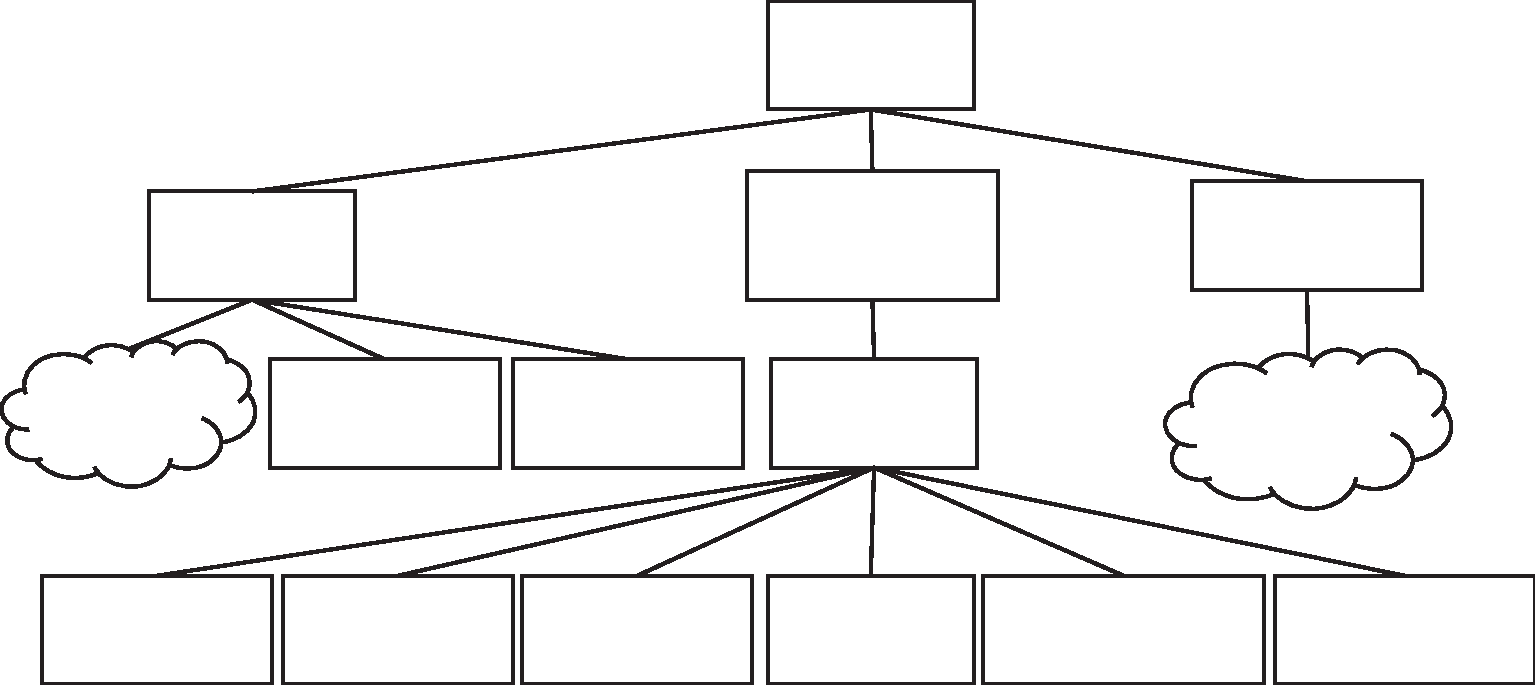
\includegraphics[angle=90,width=8.5 cm]{Bilagor/bilaga-eps-converted-to.pdf}\centering

\section{} \label{hello:bilaga}
\lstset{tabsize=2,breaklines=true,numbers=left,basicstyle=\footnotesize,xleftmargin=30pt}
\lstinputlisting[language=C,]{Kod/helloWorld.c}

% Källkod kan också vara bilaga Källkod, programspråket C inkluderas från filen helloWorld.c som ligger i mappen Kod. Läs  vilka språk som stöds http://en.wikibooks.org/wiki/LaTeX/Source_Code_Listings


% Bilagor hanvisas med \ref{Foretag:koncern} i den löpande texten.
% Exempel: man hänvisa till en bilaga. Se \ref{Foretag:koncern} för mer information.
% kommer att skrivas som:
%m an hanvisa till en bilaga. Se Bilaga A for mer information.

% texten Bilaga A kommer då bli klickbar



\end{document}
